\documentclass[conference]{IEEEtran}
\IEEEoverridecommandlockouts
% The preceding line is only needed to identify funding in the first footnote. If that is unneeded, please comment it out.
\usepackage{cite}
\usepackage{amsmath,amssymb,amsfonts}
\usepackage{algorithmic}
\usepackage{graphicx}
\usepackage{textcomp}
\usepackage{xcolor}
\def\BibTeX{{\rm B\kern-.05em{\sc i\kern-.025em b}\kern-.08em
    T\kern-.1667em\lower.7ex\hbox{E}\kern-.125emX}}
\begin{document}

\title{Projektbericht: Spotify Analyse\\}

\author{\IEEEauthorblockN{1\textsuperscript{st} Eric Kaufmann}
\IEEEauthorblockA{
Jena, Germany \\
eric.kaufmann@uni-jena.de}
\and
\IEEEauthorblockN{2\textsuperscript{nd} Maria Gogolev}
\IEEEauthorblockA{
Jena, Germany \\
maria.gogolev@uni-jena.de}
}

\maketitle

\begin{abstract}
In diesem Projektbericht wurden zwei Datensätze von Kaggle verwendet, verbunden und anschließend analysiert. Dabei werden Merkmale von Songs durch die Einteilung in Playlisten betrachtet. Mittels Erstellung einer neuen Metrik können Eigenschaften populärer Songs bestimmt und Veränderungen im Laufe der Zeit verglichen werden.
\end{abstract}

% \begin{IEEEkeywords}
% component, formatting, style, styling, insert
% \end{IEEEkeywords}

\section{Datensätze}

Als Datensätze wurden zwei von kaggle.com verwendet:
\begin{enumerate}
    \item Spotify 1.2M+ Songs\footnote{siehe https://www.kaggle.com/datasets/rodolfofigueroa/spotify-12m-songs}
    \item Spotify Playlists\footnote{siehe https://www.kaggle.com/datasets/andrewmvd/spotify-playlists}
\end{enumerate}
Ersteres besteht, wie der Name es schon verdeutlicht, aus ca. 1.2 Millionen (1,204,025 genau) unterschiedlichen Spotify Songs. Zu jedem Song sind dabei 24 Eigenschaften gegeben. Eine Auflistung aller Eigenschaften mit Beschreibung ist in Tabelle \eqref{tab:song_feat} zu finden. Der Datensatz liegt als CSV vor umfasst ungefähr 346MB. Die Daten wurden dabei mittels der offiziellen Spotify-API generiert. Jeder Song kann mittels einer eindeutigen ID beschrieben werden. Durch eine GET-Anfrage auf \textit{https://api.spotify.com/v1/tracks/\{id\}} können Informationen zum Album, Songtitel, Artisten und Publikationsdatum extrahiert werden. Mittels zweiter GET-Anfrage auf \textit{https://api.spotify.com/v1/audio-features/\{id\}} können die restlichen Eigenschaften, wie \textit{danceability}, \textit{energy} oder \textit{liveness} bestimmt werden.

\begin{table}[h]
    \caption{Beschreibung der Spalten des Spotify 1.2M+ Songs Datensatz}
    \begin{center}  
    \begin{tabular}{ll}
        Eigenschaft & Beschreibung \\ \hline
        id & Song-ID \\
        name & Songtitel \\
        album & Albumtitel \\
        album\_id &  Album-ID\\
        artists & Liste der Artisten \\
        artists\_ids & Liste der Artisten-IDs \\
        track\_number & Tracknummer des Songs im Album \\
        disc\_number & Albumnummer \\
        explicit & Song ist explicit\\
        danceability & Eignung des Songs zum tanzen ($\in [0,1]$) \\
        energy & Intensität und Aktivität des Songs ($\in [0,1]$) \\
        key & Tonart \\
        loudness & Lautstärke (dB) \\
        mode & Modus (Dur/Moll) \\
        speechiness & Sprachanteil ($\in [0,1]$) \\
        acousticness & Akustik eines Songs ($\in [0,1]$) \\
        instrumentalness & Instrumentalanteil ($\in [0,1]$) \\
        liveness & Wahrscheinlichkeit einer Liveübertragung ($\in [0,1]$) \\
        valence & Wertigkeit ($\in [0,1]$, 0=negativ und 1=positiv) \\
        tempo & Tempo (BPM) \\
        duration\_ms & Dauer (ms) \\
        time\_signature & Taktart \\
        year & Veröffentlichungsjahr \\
        release\_date & Veröffentlichungsdatum (YYYY-MM-DD)
    \end{tabular}
    \end{center}
    \label{tab:song_feat}
\end{table}

Der Datensatz ermöglicht es Songs anhand von Eigenschaften zu sortieren. Beispielsweise kann man verschiedene Eigenschaften wie die \textit{danceability}, \textit{valence} oder \textit{energy} der Songs über die Zeit betrachten. Eine andere exemplarische Anwendungsmöglichkeit ist ein Algorithmus zur Songempfehlung, bei dem man Songs mit ähnlichen Eigenschaften versucht zu verbinden. 

Um die Songs besser unterteilen zu können wurde in dieser Analyse ein zweiter Datensatz verwendet, der Spotify Playlist Datensatz. Dieser besteht aus ca. 2.8 Millionen unterschiedlichen Songs, die in ca. 162 Tausend Playlists von ungefähr 16 Tausend User eingeteilt sind. Trotz einer Größe von ca. 1.8 GB ist der Aufbau des Datensatzes recht einfach. Wie in Tabelle \eqref{tab:feat_playlist} erkennbar besitzt der Datensatz nur vier Spalten. Dabei hat ein User mit einer \textit{user\_id} eine Playlist mit der Playlistbezeichnung \textit{playlistname} angelegt. Songs, bestimmt durch den \textit{trackname} und \textit{artistname}, können somit einer Playlist zugehörig sein. Selbstverständlich können dabei Songs mehrfach vorkommen, wenn sie beispielsweise in unterschiedlichen Playlists enthalten sind oder in einer Playlist sogar mehrfach aufkommen.

\begin{table}[h]
    \caption{Beschreibung der Spalten des Spotify Playlist Datensatz}
    \begin{center}  
    \begin{tabular}{ll}
        Eigenschaft & Beschreibung \\ \hline
        user\_id & User-ID eines Spotify Nutzers \\
        artistname & Name des Artisten \\
        trackname & Songtitel \\
        playlistname & Playlistbezeichnung
    \end{tabular}
    \end{center}
    \label{tab:feat_playlist}
\end{table}

Mögliche Anwendungsfelder dieser Playlist ist beispielsweise die Untersuchung der Popularität einiger Songs durch die Anzahl der Aufkommen des Liedes in unterschiedlichen Playlisten. Mehr dazu später. 

Um die Songeigenschaften des ersten Datensatzes mit den Playlisteinteilungen des zweiten Datensatzes zu verbinden, müssen die beiden Datensätze verbunden werden. Dafür versuchen wir an den Playlist-Datensatz mittels left-join die Eigenschaften anzuheften. Dabei sollen die gemeinsamen Schlüssel der Songtitel mit Artisten sein. Um dies zu erreichen müssen jedoch vorher die Daten vorbereitet werden. Dafür wurden zunächst die Spaltennamen \textit{name} und \textit{artists}, beim Spotify 1.2M+ Datensatz, bzw. \textit{trackname} und \textit{artistname}, beim Spotify Playlistdatensatz, vereinfacht und in \textit{track} und \textit{artist} umbenannt. Somit sind die beiden Schlüssel gleich bezeichnet. 

Der nächste Schritt ist es die Liste von Artisten, welche in jeder Zeile der \textit{artist}-Spalte beim Spotify 1.2M+ Songs Datensatz zu finden ist, aufzusplitten. Diese haben nämlich eine folgende Form:

$$
    [\text'\text{artist}_1\text', \text'\text{artist}_2\text', \dots, \text'\text{artist}_n\text'].
$$

Ziel ist es, dass die Zeile des Datensatzes $n$-Mal repliziert wird und in jeder neuen Zeile nur der jeweilige $\text{artist}_i$ steht. Zum Schluss wurden die Datentypen aller Spalten angepasst und unrealistische Werte (z.B. Veröffentlichungsjahr 0) aussortiert. 

Nach dieser Vorbereitung der Daten ist es nun möglich den left-join des Spotify 1.2M+ Songs Datensatz an den Spotify Playlist Datensatz über die gemeinsame Schlüssel \textit{track} und \textit{artist} durchzuführen. Zur Vereinfachung der späteren Analyse wurde anschließend alle Zeilen mit \textit{NA}-Werten aus dem verbundenen Datensatz entfert. Somit werden auch alle Zeilen entfert, bei dem der Spotify Playlist Datensatz keine Werte für Songs aus dem Spotify 1.2M+ Songs Datensatz findet.

Die Verbindung der Datensätze hat jedoch einen großen Datenverlust zur Folge. Nach der Vorverarbeitung der einzelnen Datensätze sind beim Spotify 1.2M+ Songs Datensatz noch ca. 1,194,000 und beim Spotify Playlist Datensatz noch ca. 2,795,000 unterschiedliche Songs übrig. Nach dem join sind jedoch nur noch ca. 210,000 unterschiedliche Songs übrig. Die Gründe dafür sind recht unterschiedlich. Zum einen gibt es natürlich Songs, die in dem Spotify Playlist Datensatz vorkommen, jedoch nicht im Spotify 1.2M+ Songs Datensatz. Ein anderer Grund sind die Differenzen in der Bezeichnung der Werte der gemeinsame Schlüssel \textit{track} und \textit{artist}. Auf Spotify gibt es sehr häufig Songs, welche zwar einen bestimmen Artisten haben, jedoch ein anderer User dieser Song hochgeladen hat. Somit existiert zwar dieser Song, der Schlüssel \textit{artist} stimmt aber nicht überein. Generell werden zu jedem bekannten Song viele Unterschiedliche Versionen von vielen Nutzern hochgeladen. So gibt es von einem Song eine offizielle Version, ein Radio-Edit, eine Live-Version und verschiedene Remix. Auch Features mit anderen Artisten bringen häufig Probleme. Somit ist es möglich, dass ein Song im einen Datensatz die Form \textit{"song\_titel"} hat und im anderen \textit{"song\_titel (feat. artist2)"}. Im Spotify 1.2M+ Songs Datensatz sind die einzelnen Artisten als Liste gespeichert. Beim Spotify Playlist Datensatz sind diese zusammen als String gespeichert. Daraus entsteht das Problem, dass die Artisten im Playlist Datensatz die Form \textit{"artist1, artist2 and artist3"} bzw. \textit{"artist1 \& artist2"} haben können. Eine Teilung an Kommata ist aber auch nicht möglich, da es Artisten gibt, welche Kommata in ihrem offiziellen Namen haben. Somit wird die Schnittmenge der beiden Schlüsselmengen noch kleiner.

\section{Analyse und Interpretation}
In diesem Kapitel werfen wir einen Blick auf interessante Statistiken der Musik auf Spotify. Speziell werden wir uns anschauen wie sich Musik im Laufe der Jahre verändert, und welche Eigenschaften beliebte Lieder haben.
\subsection{Entwicklung der Musik über die Zeit}
Abbildung \ref{songs_per_year} zeigt wie viele Lieder nach dem Datenverlust pro Jahr übrig bleiben. Wir stellen fest, dass es für einige Jahre keine Einträge mehr gibt, und dass generell viel weniger ältere als moderne Lieder für unsere Analyse zur Verfügung stehen. Für die folgende Analyse ist es also wichtig zu erwähnen, dass die Ergebnisse für ferner in der Vergangenheit liegende Musik weniger zuverlässig sind.
\begin{figure*}[t]
\centering
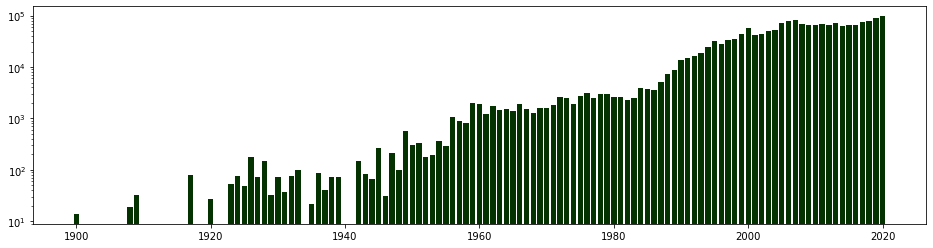
\includegraphics[width=\textwidth]{images/songs_per_year.png}
\caption{Eine logarithmisch skalierte Darstellung der Anzahl der Lieder pro Jahr.}
\label{songs_per_year}
\end{figure*}
\begin{figure*}[t]
\centering
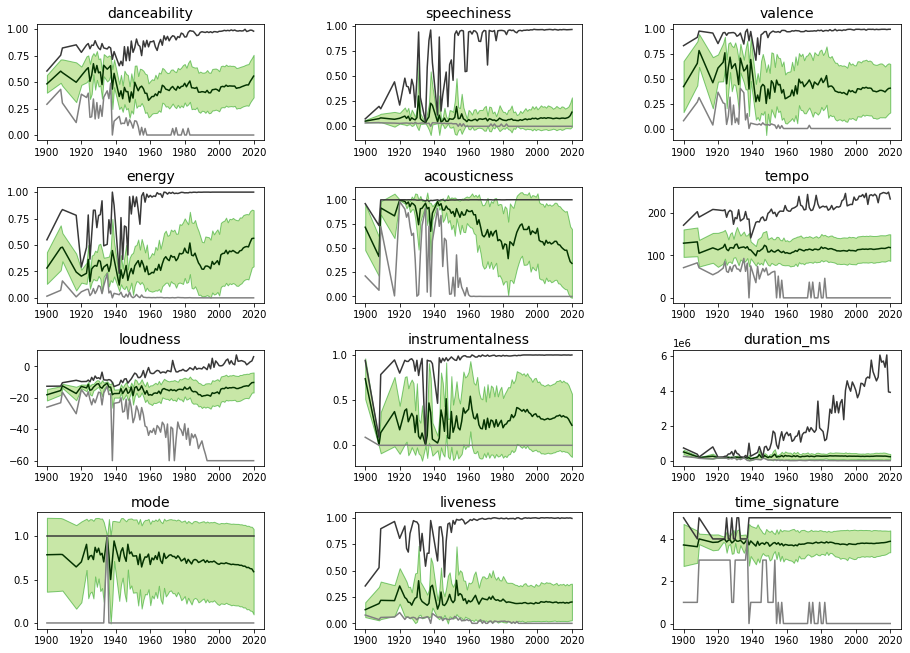
\includegraphics[width=\textwidth]{images/over_time.png}
\caption{Entwicklung der Musik-Attribute von 1900 bis 2020. Die in der Mitte verlaufende Linie ist der Durchschnittswert, die obere Linie das Maximum, die untere Linie das Minimum und der grüne Bereich ist die Standardabweichung im gegebenen Jahr.}
\label{time}
\end{figure*}
Aus den vorliegenden Daten geht hervor, dass sich die Musik im Laufe der Jahre in Bezug auf verschiedene Attribute deutlich verändert hat, und gewisse Trends ersichtlich sind. Die Analyse bezieht sich auf Abbildung \ref{time}. Im Folgenden werden nicht alle Attribute aufgegriffen, da bei ihnen Statistiken wie Standardabweichung und Durchschnittswert weniger aussagekräftig sind (bspw "Key" also der Notenschlüssel).

\begin{itemize}
\item{Danceability} Beginnend mit der danceability sehen wir, dass der Minimal- und Maximalwert über die Jahre leicht auseinander gehen. Nach einem Absinken der danceability in den 1940 Jahren zeigt der Durchschnittswert wieder einen leichten Aufwärtstrend. Die Standardabweichung bleibt relativ stabil über die Zeit.

\item{Energy} Auch bei der Energie ist ein ähnlicher Trend zu beobachten: Der Minimalwert bleibt relativ konstant, der Maximalwert steigt stetig an, der Durchschnittswert zeigt einen Aufwärtstrend und die Standardabweichung nimmt im Laufe der Zeit zu. Dies deutet darauf hin, dass die Musik im Laufe der Jahre energiegeladener geworden ist, es gleichzeitig aber mehr Diversität in diesem Attribut gibt.

\item{Loudness} Bei der Lautstärke ist ein sinkender Minimalwert und eine leichre Zunahme des Maximalwerts und Durchshcnittswertes zu verzeichnen. Musik wird also leicht lauter.

\item{Mode} Der Durchschnittswert des Modus bleibt über die gesamte Zeit überhalb von 0.5, was aussagt, dass stets mehr Musik in Dur produziert wird als in Moll, wobei ein leichter Abstieg des Durchschnittswertes in den letzten jahren zu verzeichnen ist. Es wurde also in den letzten Jahren mehr in Moll produziert.

\item{Speechiness} Das Minimum des Sprachanteils bleibt nahe bei 0, da Instrumentalmusik früher wie auch heute relevant ist. Der anfangs geringe Maximalwert entwickelt sich hingegen nach oben. Durchschnittswert und Standardabweichung bleiben gering was darauf hindeutet das der Großteil der Musik nach wie vor instrumental ist. Ansonsten zeigt die Sprachlichkeit keinen starken Trend.

\item{Acousticness} Die Akustizität zeigt über die Jahre einen Rückgang der Durchschnittswerte, was darauf hindeutet, dass die Musik im Laufe der Jahre elektronischer geworden ist. Die Standardabweichung für das Attribut "Akustizität" nimmt im Laufe der Zeit zu, was darauf hindeutet, dass die Verteilung der Akustizitätswerte im Laufe der Zeit immer vielfältiger und unterschiedlicher wird. Elektronische Musik ersetzt akustische Musik also nicht, sondern kommt zusätzlich hinzu. 

\item{instrumentalness} Bei der Instrumentalität ist ein auf und ab zu sehen, ohne klaren Trend hinsichtlich wachsendem oder fallendem Instrumentalanteil. Die Standardabweichung bleibt konsistent hoch, was bedeutet, dass nach wie vor viele Lieder mit hohem als auch niedrigem Instrumentalanteil produziert werden.

\item{liveness} Auch "Liveness" zeigt keinen eindeutigen Trend. Der Durchschnittswert ist relativ niedrig mit einer geringen Standardabweichung, was darauf hindeutet dass der Großteil der Musik nicht live übertragen wurde.

\item{valence} Die Valenz zeigt keinen konstanten Abstieg der Statistiken, aber einen Reduktion des Durchschnittswerts ab den 1940ern ähnlich zur "Danceability", was darauf hindeutet, dass die Musik seit dieser Zeit weniger positiv ist.

\item{Tempo} Das Maximaltempo wird über die Jahre höher und das Minimaltempo wird niedriger während der Durchschnittswert relativ konstant im mittleren Bereich der Attributskala bleibt. Die Standardabweichung ist niedrig und konstant. Die meisten Lieder sind also weder langsam noch schnell, aber es wird über die Jahre immer wieder mit neuen Tempo-Rekorden experimentiert.

\item{Duration} Die Dauer zeigt einen starken Anstieg des Maximalwertes. Minimal- und Durchschnittswerte bleiben relativ konsistent und gering, genauso wie die Standardabweichung. Die Musik ist in Bezug auf die Dauer eher stabil und vorhersehbar.

\item{Time signature} Der Anteil der Songs mit 4/4-Takt ist im Laufe der Zeit relativ stabil geblieben, die meisten Songs sind im 4/4-Takt, die Standardabweichung der Taktart ist gering und im Laufe der Zeit stabil, was darauf hindeutet, dass die meisten Songs, nach wie vor, hauptsächlich 4 Schläge pro Takt haben.
\end{itemize}

Insgesamt erweckt die Grafik den Anschein, dass die Musik im Laufe der Jahre energiegeladener und etwas tanzbarer und lauter geworden ist, wobei die durchschnittliche Tanzbarkeit und das Energieniveau allmählich gestiegen sind. Die durchschnittliche Akustik und Instrumentalität schwanken. Die Musik scheint aber insgesamt zu mehr elektronischen oder synthetischen Klängen zu tendieren, da sich der Anteil der akustischen Musik über die Jahre eindeutig verringert. Für die Attribute deren Durchschnittswert einem klaren Trend folgt, also der relative Rückgang akustischer Elemente und der Anstieg der Energie, lässt sich auch ein Anstieg in der Standardabweichung, also der Diversität in der Ausprägung des Attributs feststellen.

\subsection{Popularität}
Das Ziel in diesem Abschnitt besteht darin, die Statistiken der Attribute durchschnittlicher Lieder und Künstler mit den Statistiken populärer Lieder Künstler zu vergleichen, um herauszufinden was Popularität ausmacht.
In keinem der beiden Datensätzen gibt es Informationen über die Beliebtheit, weshalb wir zunächst ein Beliebtwert für jeden Künstler und für jeden Song wie folgt ausrechnen: Es wird gezählt wie oft das gegebene Lied/ der gegebene Künstler in Playlisten aufgenommen wurde. Das gibt dann einen Schätzwert für die Popularität. 
In Tabelle \ref{tab:topsongs} sieht man die 10 Lieder die am häufigsten in Playlisten vorkommen, und Tabelle \ref{tab:topartists} zeigt die top 10 Künstler die am häufigsten in Playlisten aufgenommen wurden.
Abbildung \ref{popularity_time} zeigt wie oft im Durchschnitt ein Lied welches im gegebenen Jahr veröffentlicht wurde, in Playlists erschien. Es lässt sich feststellen, dass besonders Musik aus den letzten Jahren sehr populär ist.

\begin{table}[h]
\centering
\begin{tabular}{c c c c} 
\hline
track & artist & count \\ [0.5ex] 
\hline
Ho Hey & The Lumineers & 1547 \\ 
Kids & MGMT & 1319 \\ 
Rather Be (feat. Jess Glynne) & Clean Bandit & 1279 \\ 
Do I Wanna Know? & Arctic Monkeys & 1204 \\ 
Chandelier & Sia & 1169 \\ 
Don't Stop Believin' & Journey & 1114 \\ 
Sail & AWOLNATION & 1110 \\ 
Take Me Out & Franz Ferdinand & 1084 \\ 
Creep & Radiohead & 1066 \\ 
Summer & Calvin Harris & 1058 \\ [1ex] 
\hline
\end{tabular}

\caption{Top 100 populärste Lieder}
\label{tab:topsongs}
\end{table}

\begin{table}[h]
\centering
\begin{tabular}{c c} 
\hline
artist & count \\ [0.5ex] 
\hline
Beyoncé & 3476 \\ 
Radiohead & 3406 \\ 
Arctic Monkeys & 3038 \\ 
Coldplay & 2855 \\ 
Michael Jackson & 2593 \\ 
MGMT & 2516 \\ 
Bob Dylan & 2307 \\ 
Foo Fighters & 2212 \\ 
The Strokes & 2189 \\ 
Bruce Springsteen & 2131 \\ [1ex] 
\hline
\end{tabular}
\caption{Top 100 populärste Künstler}
\label{tab:topartists}
\end{table}
\subsubsection{Vergleich populärer Lieder mit durchschnittlichen Liedern}

\begin{figure*}[t]
\centering
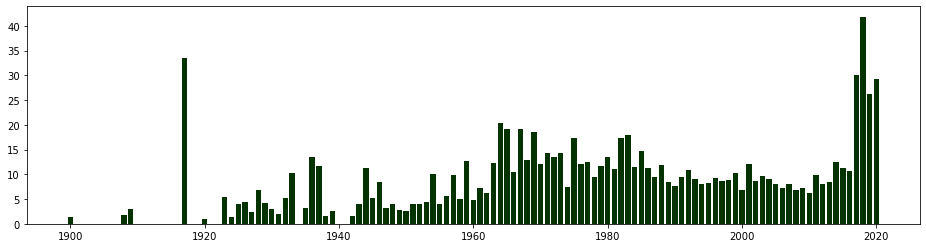
\includegraphics[width=\textwidth]{images/popularity_per_year.png}
\caption{Durchschnittliche Beliebtheit der im gegebenen Jahr veröffentlichten Musik.}
\label{popularity_time}
\end{figure*}

\begin{figure*}[t]
\centering
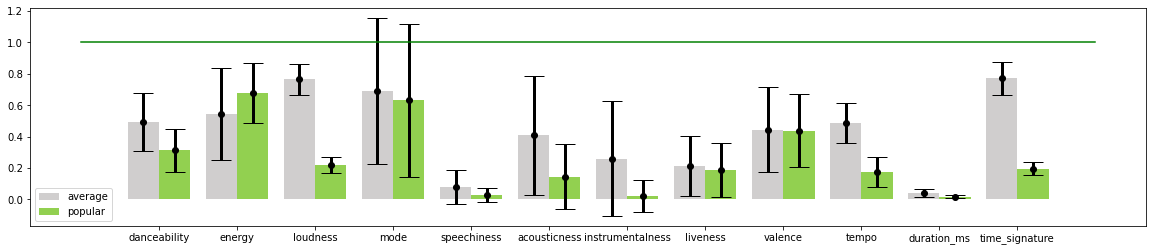
\includegraphics[width=\textwidth]{images/pop_tracks.png}
\caption{Vergleich des Durchschnittswerts und der Standardabweichungen verschiedener Attribute der den Top 100 beliebtesten Songs mit allen Songs. Rechts (grün) sind die populären Lieder dargestellt, und links(grau) sieht man die durchschnittlichen Lieder. Da die Attribute unterschiedliche Wertebereiche haben, werden die Durchschnittswerte und die Standardabweichungen jeweils mit dem globalen Maximum und dem globalen Minimum des Attributs skaliert.}
\label{popular tracks}
\end{figure*}

In Abbildung \ref{popular tracks} wird deutlich, dass die Durchschnittswerte der populären Songs wesentlich niedriger für "Danceability", für die Lautstärke, für akustische Elemente, für Tempo und für die Taktart. Das heißt populäre Lieder eignen sich im Durchschnitt weniger zum Tanzen, sind viel leiser, langsamer, und haben einen geringeren akustischen Anteil. Sie haben weniger Schläge pro Takt. Populäre Songs sind jedoch energetischer, was logisch erscheint, da die durchschnittliche Energie (siehe Abb. \ref{time}) und die durchschnittliche Beliebtheit (siehe Abb. \ref{popularity_time}) in den letzten Jahren besonders hoch ist.
Außerdem kann man erkennen, dass die Standardabweichung für die top 100 beliebtesten Lieder in fast allen Attributen geringer ist, was darauf hindeutet, dass sich populäre Lieder untereinander in ihren Attributen ähnlicher sind.
Man kann auf Grund dieser Resultate populäre Lieder (Lieder die oft in Playlisten auf Spotify aufgenommen werden) wie folgt charakterisieren: sie haben trotz geringerem Tempo und geringer Lautstärke viel Energie leicht positiver, und generell weniger Variation in den Attributen. Eventuell eignen sie sich also eher zum Hören im Hintergrund. 

\subsubsection{Vergleich populärer Künstler mit durchschnittlichen Künstlern}

Zunächst haben wir die Durchschnittswerte für jeden Künstler und jedes Attribut durch Aggregation aller Lieder des Künstlers über das arithmetische Mittel errechnet. Dannach wurden die top 100 beliebtesten Künstler gefiltert, und mit allen Künstlern insgesamt verglichen.

\begin{figure*}[t]
\centering
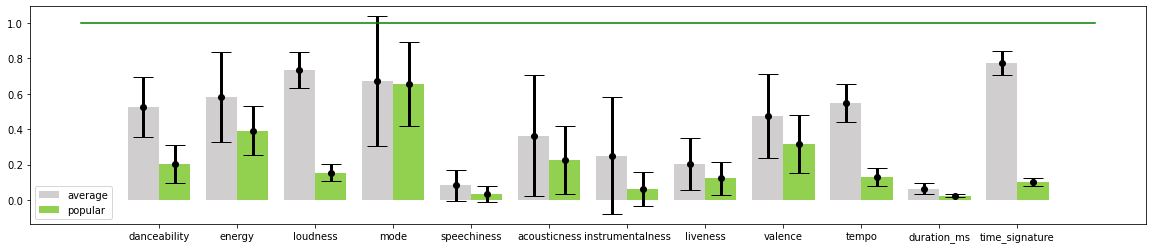
\includegraphics[width=\textwidth]{images/pop_arts.png}
\caption{Vergleich des Durchschnittswerts und der Standardabweichungen verschiedener Attribute der den Top 100 beliebtesten Künstler mit allen Künstlern insgesamt. Rechts (grün) sind die populären Künstler dargestellt, und links(grau) sieht man die durchschnittlichen Artisten. Da die Attribute unterschiedliche Wertebereiche haben, werden die Durchschnittswerte und die Standardabweichungen jeweils mit dem globalen Maximum und dem globalen Minimum des Attributs skaliert.}
\label{popular artists}
\end{figure*}
In Abbildung \ref{popular artists} sieht man viele Ähnlichkeiten zu den Ergebnissen in Abbildung \ref{popular tracks}.

Ein paar kleinere Unterschiede sind die im Durchschnitt geringere "Valence" der populären Künstler im Vergleich zum Durchschnittskünstler und die Ähnlchkeit der durchschnittlichen Energielevel. Die kleine Standardabweichung ist auch hier wieder indikativ für die Ähnlichkeit der populären Künstler untereinander.
Was man in beiden Abbildungen erkennen kann, ist dass Popularität mit weniger Eignung zum Tanzen, langsamerem Tempo, weniger Schlägen pro Takt, geringerer Lautstärke, weniger Instrumentalanteil, weniger akustischen Elementen und weniger Varianz in den Attributen einhergeht.

\subsubsection{Vergleich der Eigenschaften populärer Lieder mit den Liedern populärer Künstler}
In Abbildung \ref{popular artists vs popular songs} sieht man die Statistiken beliebter Künstler gegenübergestellt zu den Statistiken beliebter Lieder. Man kann folgende Unterschiede feststellen: Die Varianz der Attribute scheint bei beliebten Künstlern noch stärker eingeschränkt zu sein als bei den beliebtesten Songs, was bedeutet dass sich beliebte Künstler untereinander mehr ähneln als beliebte Lieder. Weiterhin haben beliebte Künstler etwas weniger energetische Lieder, aber dafür mit höherem Akustik-Anteil.

\begin{figure*}[t]
\centering
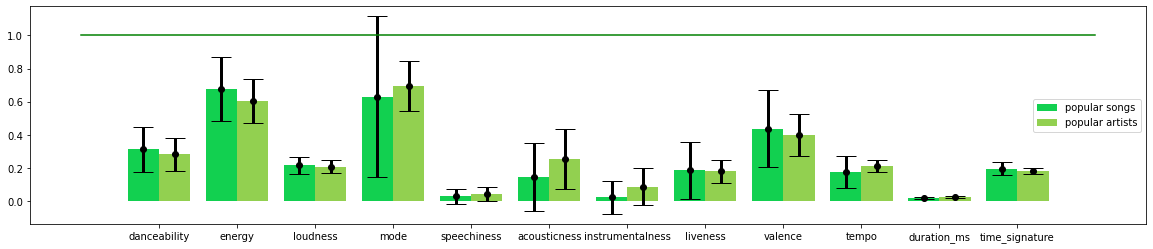
\includegraphics[width=\textwidth]{images/tracks_arts.png}
\caption{Vergleich des Durchschnittswerts und der Standardabweichungen verschiedener Attribute der Durchschnittssongs der Top 100 beliebtesten Künstler mit den top 100 beliebtesten Songs insgesamt. Rechts (grün) sind die populären Künstler dargestellt, und links sieht man die populären Songs. Da die Attribute unterschiedliche Wertebereiche haben, werden die Durchschnittswerte und die Standardabweichungen jeweils mit dem globalen Maximum und dem globalen Minimum des Attributs skaliert.}
\label{popular artists vs popular songs}
\end{figure*}


\begin{thebibliography}{00}
\bibitem{d1} Pichl, Martin; Zangerle, Eva; Specht, Günther: "Towards a Context-Aware Music Recommendation Approach: What is Hidden in the Playlist Name?" in 15th IEEE International Conference on Data Mining Workshops (ICDM 2015), pp. 1360-1365, IEEE, Atlantic City, 2015.
\bibitem{d2} Figueroa, Rodolfo. (2020). Spotify 12M Songs [Dataset]. Kaggle. https://www.kaggle.com/datasets/rodolfofigueroa/spotify-12m-songs

\bibitem{b1} G. Eason, B. Noble, and I. N. Sneddon, ``On certain integrals of Lipschitz-Hankel type involving products of Bessel functions,'' Phil. Trans. Roy. Soc. London, vol. A247, pp. 529--551, April 1955.
\bibitem{b2} J. Clerk Maxwell, A Treatise on Electricity and Magnetism, 3rd ed., vol. 2. Oxford: Clarendon, 1892, pp.68--73.
\bibitem{b3} I. S. Jacobs and C. P. Bean, ``Fine particles, thin films and exchange anisotropy,'' in Magnetism, vol. III, G. T. Rado and H. Suhl, Eds. New York: Academic, 1963, pp. 271--350.
\bibitem{b4} K. Elissa, ``Title of paper if known,'' unpublished.
\bibitem{b5} R. Nicole, ``Title of paper with only first word capitalized,'' J. Name Stand. Abbrev., in press.
\bibitem{b6} Y. Yorozu, M. Hirano, K. Oka, and Y. Tagawa, ``Electron spectroscopy studies on magneto-optical media and plastic substrate interface,'' IEEE Transl. J. Magn. Japan, vol. 2, pp. 740--741, August 1987 [Digests 9th Annual Conf. Magnetics Japan, p. 301, 1982].
\bibitem{b7} M. Young, The Technical Writer's Handbook. Mill Valley, CA: University Science, 1989.
\end{thebibliography}
\vspace{12pt}
\color{red}
IEEE conference templates contain guidance text for composing and formatting conference papers. Please ensure that all template text is removed from your conference paper prior to submission to the conference. Failure to remove the template text from your paper may result in your paper not being published.

\end{document}
